\begin{figure}[htbp]
\centering
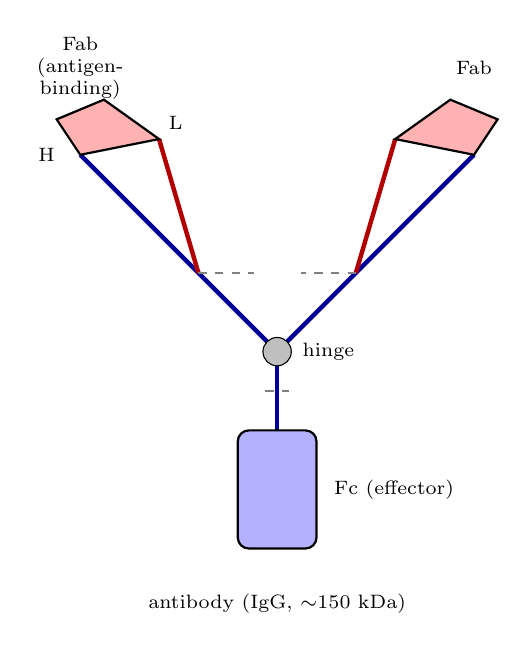
\begin{tikzpicture}[scale=1.0, every node/.style={font=\small}]
  % Heavy chains
  \draw[ultra thick, blue!60!black] (-2.5,2.5) -- (0,0) -- (2.5,2.5);
  \draw[ultra thick, blue!60!black] (0,0) -- (0,-2.5);
  % Light chains
  \draw[ultra thick, red!70!black] (-1.5,2.7) -- (-1.0,1.0);
  \draw[ultra thick, red!70!black] (1.5,2.7) -- (1.0,1.0);
  % Variable regions (Fab tips)
  \draw[fill=red!30, thick] (-2.5,2.5) -- (-2.8,2.95) -- (-2.2,3.2) -- (-1.5,2.7) -- cycle;
  \draw[fill=red!30, thick] (2.5,2.5) -- (2.8,2.95) -- (2.2,3.2) -- (1.5,2.7) -- cycle;
  % Fab labels
  \node[align=center, font=\scriptsize] at (-2.5,3.6) {Fab\\(antigen-\\binding)};
  \node[align=center, font=\scriptsize] at (2.5,3.6) {Fab};
  % Fc region
  \draw[fill=blue!30, thick, rounded corners=4pt] (-0.5,-2.5) rectangle (0.5,-1.0);
  \node[right, font=\scriptsize] at (0.6,-1.75) {Fc (effector)};
  % Hinge
  \draw[fill=gray!50] (0,0) circle (0.18);
  \node[right, font=\scriptsize] at (0.2,0) {hinge};
  % Disulfide bonds
  \draw[thick, gray, dashed] (-1.0,1.0) -- (-0.3,1.0);
  \draw[thick, gray, dashed] (1.0,1.0) -- (0.3,1.0);
  \draw[thick, gray, dashed] (-0.15,-0.5) -- (0.15,-0.5);
  % Chain labels
  \node[left, font=\scriptsize] at (-2.7,2.5) {H};
  \node[right, font=\scriptsize] at (-1.5,2.9) {L};
  % Annotation
  \node[align=center, font=\scriptsize] at (0,-3.2) {antibody (IgG, $\sim$150 kDa)};
\end{tikzpicture}
\caption[Antibody structure]{Schematic Y-shaped structure of an IgG
antibody. Two identical heavy chains (blue) and two identical light
chains (red) form a hinged structure. The Fab arms carry the
variable-region antigen-binding sites generated by somatic V(D)J
recombination; the Fc stem mediates effector functions
(complement activation, binding to Fc receptors on phagocytes and
mast cells).}
\label{fig:vol06:ch07:antibody}
\end{figure}
